
\paragraph{The correctness of distributed algorithms} is the focus of this thesis. Distributed algorithms
are algorithms that are designed to run on multiple processors, without centralized control. They play a crucial role in modern computing.
For example, they control machines that we use on a daily basis such as smartphones, but also critical systems such as medical devices, trains, airplanes, and spaceships. Errors in distributed algorithms can have severe consequences, such as the loss of critical data or even the loss of human life. Ensuring their correctness is vital but challenging due to the inherent complexity of these systems~\cite{heiser2010theroad, lamport2019thebyzantine}. 

The Needham-Schroeder protocol~\cite{needham1978using}\textemdash a well-known distributed algorithm for two computers to verify each other's identity\textemdash exemplifies this challenge: it was found to have serious security flaws~\cite{lowe1996breaking} 17 years after it was published~\cite{cortier2014formal}.
To address the challenge of uncovering subtle vulnerabilities in distributed algorithms, one natural approach is to test all possible scenarios. This applies if the number of scenarios is small, infeasible otherwise. 
This gap motivates the use of formal verification, and in particular, Interactive Theorem Proving.

\paragraph{Interactive Theorem Proving (ITP)} provides a rigorous framework for formal verification via human-guided collaboration with proof assistants~\cite{moura2021lean4,nipkow2002isabelle,bertot2004coq}. In this paradigm, distributed algorithms are formally modeled as mathematical structures, with their properties expressed as mathematical statements. The verification process involves guiding proof assistants through a sequence of reasoning steps to construct a mathematical proof that the algorithm satisfies the desired properties. The proof assistant checks the correctness of each step, ensuring that the final proof is valid. This approach
can tackle the challenge of verifying distributed algorithms even if the number of scenarios is infinite. It allows for a high degree of confidence in the correctness of the distributed algorithm, as it is based on rigorous mathematical reasoning~\cite{potop2019formal,courtieu2016certified}. 

However, ITP presents two challenges. Firstly, it demands a deep understanding of both the system being verified and the proof assistant being used. Secondly, the proof construction process remains inherently labor-intensive because the proof assistant must be guided through each reasoning step and every possible case must be addressed in detail.
While modern proof assistants incorporate increasingly sophisticated automation for proof construction, fundamental limitations arise from the inherent undecidability of expressive logics.
Consequently, complete automation of proof construction for non-trivial distributed systems remains theoretically impossible. Nevertheless, well-designed automated techniques can significantly reduce the verification effort.

\paragraph{Automated techniques} are developed for verifying specific properties of systems~\cite{contejean2011automated,giesl2014proving,blanchet2016modeling}. They automatically check conditions that imply the properties of interest, where these conditions are often easy to verify.
% Similar to checking the derivative $f'(x) = 2x$ is non-negative for all $x \in \mathbb{R}$, to ensure the monotonic increase of the function $f(x) = x^2$ for all $x \in \mathbb{R}$.
These techniques are typically implemented as tools accessible to non-experts in formal methods while also accelerating verification for experts. To ensure the correctness of the result obtained by the tool, some tools can generate certificates that can be checked by proof assistants.
These techniques provide a practical alternative to interactive theorem proving.
To develop such automated methods, distributed algorithms need to be modeled
using a formalism that enables rigorous analysis
and automated verification of their properties. 
% In this thesis, we focus on modeling distributed algorithms using graph transformation.

\paragraph{Finite edge-labeled directed multigraphs} model distributed algorithms in this thesis. This formalism extends directed graphs by allowing multiple edges between nodes and labeled edges. Computation units are represented by nodes; communication channels are represented by edges; states of the system are modeled by graphs whose edges have labels representing information encoded in computation units and states of communication channels. For example, consider the graph in~\autoref{fig:graph_modeling_state_network} which models a distributed network with six computation units.
 \begin{figure}[!htbp]
        \centering
        \resizebox{0.3\textwidth}{!}{
                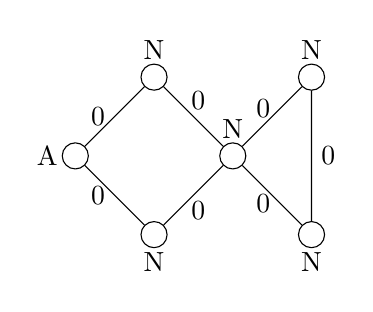
\begin{tikzpicture}
                    \node[draw, circle] (n1) at (0,0) {};
                    \node[draw, circle] (n2) at (1,1) {};
                    \node[draw, circle] (n4) at (1,-1) {};
                    \node[draw, circle] (n3) at (2,0) {};
                    \node[draw, circle] (n5) at (3,-1){};
                    \node[draw, circle] (n6) at (3,1){};
                    \draw[-] (n1)--(n2)--(n3)--(n4);
                    \draw[-] (n4)--(n1);
                    \draw[-] (n3)--(n6)--(n5)--(n3);
                    \draw[transparent, rounded corners,rotate around={45:(0,-0.5)}, dotted] (0,-0.5) rectangle (2.2,0.3) ;
                    \draw[transparent, rounded corners,rotate around={-45:(0,0.5)}, dotted] (0,0.5) rectangle (2.2,-0.3) ;   
                    \draw(-0.1,0) node[left] {A};
                    \draw(1,1.1) node[above] {N};
                    \draw(1,-1.1) node[below] {N};
                    \draw(2,0.1) node[above] {N};
                    \draw(3,1.1) node[above] {N};
                    \draw(3,-1.1) node[below] {N};
                    % edge labels
                    \draw(1.35,0.7) node[right] {0};
                    \draw(1.35,-0.7) node[right] {0};
                    \draw(0.5,0.5) node[left] {0};
                    \draw(0.5,-0.5) node[left] {0};
                    \draw(2.6,0.6) node[left] {0};
                    \draw(2.6,-0.6) node[left] {0};
                    \draw(3,0) node[right] {0};
                \end{tikzpicture}
    }
    \caption{A graph modeling a network configuration}
    \label{fig:graph_modeling_state_network}
\end{figure}
Each node represents a computation unit.
Formally, a unit's state is indicated by the label of its self-loop edge; for diagrammatic clarity, these self-loops are omitted and their labels are displayed directly on nodes.  
 In~\autoref{fig:graph_modeling_state_network}, one unit is active ("A") while the remaining five are neutral ("N"). Edges represent communication channels, all initially in state "0".

\paragraph{Graph transformation} provides an intuitive yet formal way to model distributed algorithms: state changes of the system are modeled by replacing subgraphs in the graph by other subgraphs according to transformation rules.
As an example, consider a distributed spanning tree construction algorithm: when an active unit ("A") detects a neutral neighbor ("N") via a channel in state "0", it activates the neighbor and updates the channel to state "1". Its behavior can be captured by a graph transformation rule, which identifies an occurrence of the graph \tikz[baseline=0ex]{ 
            \node (x) at (0,0) {$\bullet$};  
            \node (y) at (1,0) {$\bullet$};
            \draw[-] (x) -- node[midway,above] {0} (y) ;
            \node () at (0,0.3) {$A$};  
            \node () at (1,0.3) {$N$};
 } then modifies its labels to obtain an occurrence of the graph \tikz[baseline=0ex]{ 
                \node (x) at (0,0) {$\bullet$};  
                \node (y) at (1,0) {$\bullet$};
                \draw[-] (x) -- node[midway,above] {1} (y) ;
                \node () at (0,0.3) {$A$};  
                \node () at (1,0.3) {$A$};
 }. It can be illustrated as~\autoref{fig:intro:graph_transformation_rule_0} where numbers inside nodes are their identifiers.
 \begin{figure}[!htbp]
    \centering
       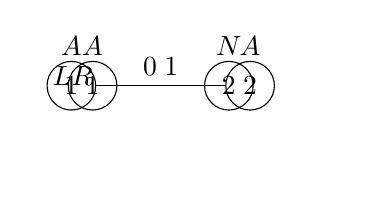
\begin{tikzpicture}
                    \graphbox{\( L \)}{0mm}{-3mm}{34mm}{15mm}{-8mm}{-9mm}{
                        \node[draw, circle] (x) at (0,0) {1};  
                        \node[draw, circle] (y) at (2,0) {2};
                        \draw[-] (x) -- node[midway,above] {0} (y) ;
                        \node  () at (0,0.5) {$A$};  
                        \node () at (2,0.5) {$N$};
                    } 
                    \graphbox{\( R \)}{40mm}{-3mm}{34mm}{15mm}{-8mm}{-9mm}{
                        \node[draw, circle]  (x) at (0,0) {1};  
                        \node[draw, circle]  (y) at (2,0) {2};
                        \draw[-] (x) -- node[midway,above] {1} (y) ;
                        \node () at (0,0.5) {$A$};  
                        \node () at (2,0.5) {$A$};
                    }  
                    \node () at (37mm,-10mm) {\( \rightarrowtail \)}; % K -> L
                \end{tikzpicture}
    \caption{}
    \label{fig:intro:graph_transformation_rule_0}
\end{figure}
A sample execution sequence starting from the configuration in~\autoref{fig:graph_modeling_state_network} is shown in~\autoref{fig:intro_sequence_of_transformation}. Upon termination, a spanning tree can be constructed using edges labeled by "1".
    \begin{figure}[!htbp]
        \centering
        \resizebox{0.3\textwidth}{!}{
                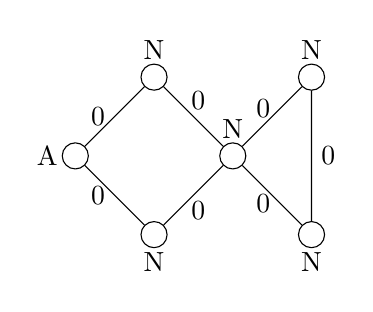
\begin{tikzpicture}
                    \node[draw, circle] (n1) at (0,0) {};
                    \node[draw, circle] (n2) at (1,1) {};
                    \node[draw, circle] (n4) at (1,-1) {};
                    \node[draw, circle] (n3) at (2,0) {};
                    \node[draw, circle] (n5) at (3,-1){};
                    \node[draw, circle] (n6) at (3,1){};
                    \draw[-] (n1)--(n2)--(n3)--(n4);
                    \draw[-] (n4)--(n1);
                    \draw[-] (n3)--(n6)--(n5)--(n3);
                    \draw[transparent, rounded corners,rotate around={45:(0,-0.5)}, dotted] (0,-0.5) rectangle (2.2,0.3) ;
                    \draw[transparent, rounded corners,rotate around={-45:(0,0.5)}, dotted] (0,0.5) rectangle (2.2,-0.3) ;   
    
                    \draw(-0.1,0) node[left] {A};
                    \draw(1,1.1) node[above] {N};
                    \draw(1,-1.1) node[below] {N};
                    \draw(2,0.1) node[above] {N};
                    \draw(3,1.1) node[above] {N};
                    \draw(3,-1.1) node[below] {N};
    
                    % edge labels
                    \draw(1.35,0.7) node[right] {0};
                    \draw(1.35,-0.7) node[right] {0};
                    \draw(0.5,0.5) node[left] {0};
                    \draw(0.5,-0.5) node[left] {0};
                    \draw(2.6,0.6) node[left] {0};
                    \draw(2.6,-0.6) node[left] {0};
                    \draw(3,0) node[right] {0};
                \end{tikzpicture}
    }
  \resizebox{0.3\textwidth}{!}{
                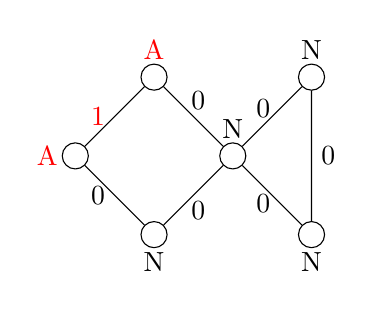
\begin{tikzpicture}
                    \node[draw, circle] (n1) at (0,0) {};
                    \node[draw, circle] (n2) at (1,1) {};
                    \node[draw, circle] (n4) at (1,-1) {};
                    \node[draw, circle] (n3) at (2,0) {};
                    
                    \node[draw, circle] (n5) at (3,-1){};
                    \node[draw, circle] (n6) at (3,1){};
        
                    \draw[-] (n1)--(n2)--(n3)--(n4);
                    \draw[-] (n4)--(n1);
                    \draw[-] (n3)--(n6)--(n5)--(n3);
        
                    \draw[transparent, rounded corners,rotate around={45:(0,-0.5)}, dotted] (0,-0.5) rectangle (2.2,0.3) ;
                    \draw[transparent, rounded corners,rotate around={-45:(0,0.5)}, dotted] (0,0.5) rectangle (2.2,-0.3) ;
    
                    \draw(-0.1,0) node[left] {\textcolor{red}{A}};
                    \draw(1,1.1) node[above] {\textcolor{red}{A}};
                    \draw(1,-1.1) node[below] {N};
                    \draw(2,0.1) node[above] {N};
                    \draw(3,1.1) node[above] {N};
                    \draw(3,-1.1) node[below] {N};
    
                    % edge labels
                    \draw(1.35,0.7) node[right] {0};
                    \draw(1.35,-0.7) node[right] {0};
                    \draw(0.5,0.5) node[left] {\textcolor{red}{1}};
                    \draw(0.5,-0.5) node[left] {0};
                    \draw(2.6,0.6) node[left] {0};
                    \draw(2.6,-0.6) node[left] {0};
                    \draw(3,0) node[right] {0};
                \end{tikzpicture}
}
\resizebox{0.3\textwidth}{!}{
                    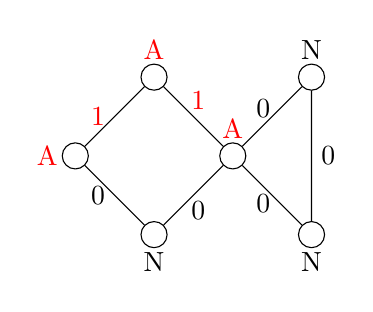
\begin{tikzpicture}
                        \node[draw, circle] (n1) at (0,0) {};
                        \node[draw, circle] (n2) at (1,1) {};
                        \node[draw, circle] (n4) at (1,-1) {};
                        \node[draw, circle] (n3) at (2,0) {};
                        
                        \node[draw, circle] (n5) at (3,-1){};
                        \node[draw, circle] (n6) at (3,1){};
            
                        \draw[-] (n1)--(n2)--(n3)--(n4);
                        \draw[-] (n4)--(n1);
                        \draw[-] (n3)--(n6)--(n5)--(n3);
            
                        \draw[transparent, rounded corners,rotate around={45:(0,-0.5)}, dotted] (0,-0.5) rectangle (2.2,0.3) ;
                        \draw[transparent, rounded corners,rotate around={-45:(0,0.5)}, dotted] (0,0.5) rectangle (2.2,-0.3) ;
    
                        \draw(-0.1,0) node[left] {\textcolor{red}{A}};
                        \draw(1,1.1) node[above] {\textcolor{red}{A}};
                        \draw(1,-1.1) node[below] {N};
                        \draw(2,0.1) node[above] {\textcolor{red}{A}};
                        \draw(3,1.1) node[above] {N};
                        \draw(3,-1.1) node[below] {N};
    
                        % edge labels
                        \draw(1.35,0.7) node[right] {\textcolor{red}{1}};
                        \draw(1.35,-0.7) node[right] {0};
                        \draw(0.5,0.5) node[left] {\textcolor{red}{1}};
                        \draw(0.5,-0.5) node[left] {0};
                        \draw(2.6,0.6) node[left] {0};
                        \draw(2.6,-0.6) node[left] {0};
                        \draw(3,0) node[right] {0};
                    \end{tikzpicture}
}


\resizebox{0.3\textwidth}{!}{
                    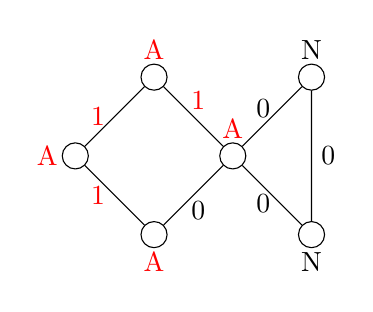
\begin{tikzpicture}
                        \node[draw, circle] (n1) at (0,0) {};
                        \node[draw, circle] (n2) at (1,1) {};
                        \node[draw, circle] (n4) at (1,-1) {};
                        \node[draw, circle] (n3) at (2,0) {};
                        
                        \node[draw, circle] (n5) at (3,-1){};
                        \node[draw, circle] (n6) at (3,1){};
            
                        \draw[-] (n1)--(n2)--(n3)--(n4);
                        \draw[-] (n4)--(n1);
                        \draw[-] (n3)--(n6)--(n5)--(n3);
            
                        \draw[transparent, rounded corners,rotate around={45:(0,-0.5)}, dotted] (0,-0.5) rectangle (2.2,0.3) ;
                        \draw[transparent, rounded corners,rotate around={-45:(0,0.5)}, dotted] (0,0.5) rectangle (2.2,-0.3) ;
    
                        \draw(-0.1,0) node[left] {\textcolor{red}{A}};
                        \draw(1,1.1) node[above] {\textcolor{red}{A}};
                        \draw(1,-1.1) node[below] {\textcolor{red}{A}};
                        \draw(2,0.1) node[above] {\textcolor{red}{A}};
                        \draw(3,1.1) node[above] {N};
                        \draw(3,-1.1) node[below] {N};
    
                        % edge labels
                        \draw(1.35,0.7) node[right] {\textcolor{red}{1}};
                        \draw(1.35,-0.7) node[right] {0};
                        \draw(0.5,0.5) node[left] {\textcolor{red}{1}};
                        \draw(0.5,-0.5) node[left] {\textcolor{red}{1}};
                        \draw(2.6,0.6) node[left] {0};
                        \draw(2.6,-0.6) node[left] {0};
                        \draw(3,0) node[right] {0};
                    \end{tikzpicture}
}
\resizebox{0.3\textwidth}{!}{
                    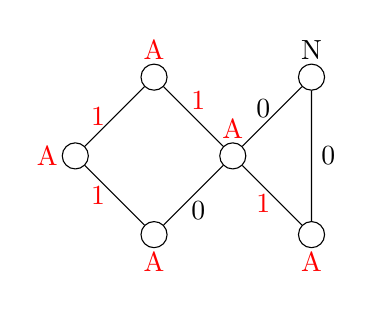
\begin{tikzpicture}
                        \node[draw, circle] (n1) at (0,0) {};
                        \node[draw, circle] (n2) at (1,1) {};
                        \node[draw, circle] (n4) at (1,-1) {};
                        \node[draw, circle] (n3) at (2,0) {};
                        
                        \node[draw, circle] (n5) at (3,-1){};
                        \node[draw, circle] (n6) at (3,1){};
            
                        \draw[-] (n1)--(n2)--(n3)--(n4);
                        \draw[-] (n4)--(n1);
                        \draw[-] (n3)--(n6)--(n5)--(n3);
            
                        \draw[transparent, rounded corners,rotate around={45:(0,-0.5)}, dotted] (0,-0.5) rectangle (2.2,0.3) ;
                        \draw[transparent, rounded corners,rotate around={-45:(0,0.5)}, dotted] (0,0.5) rectangle (2.2,-0.3) ;
              
                        \draw(-0.1,0) node[left] {\textcolor{red}{A}};
                        \draw(1,1.1) node[above] {\textcolor{red}{A}};
                        \draw(1,-1.1) node[below] {\textcolor{red}{A}};
                        \draw(2,0.1) node[above] {\textcolor{red}{A}};
                        \draw(3,1.1) node[above] {N};
                        \draw(3,-1.1) node[below] {\textcolor{red}{A}};
    
                        % edge labels
                        \draw(1.35,0.7) node[right] {\textcolor{red}{1}};
                        \draw(1.35,-0.7) node[right] {0};
                        \draw(0.5,0.5) node[left] {\textcolor{red}{1}};
                        \draw(0.5,-0.5) node[left] {\textcolor{red}{1}};
                        \draw(2.6,0.6) node[left] {0};
                        \draw(2.6,-0.6) node[left] {\textcolor{red}{1}};
                        \draw(3,0) node[right] {0};
                    \end{tikzpicture}
}
\resizebox{0.3\textwidth}{!}{
                    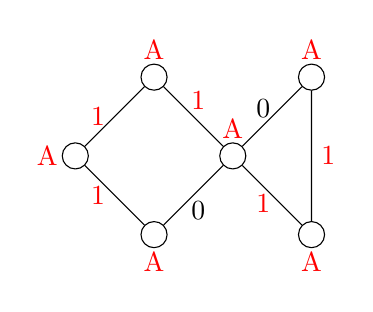
\begin{tikzpicture}
                        \node[draw, circle] (n1) at (0,0) {};
                        \node[draw, circle] (n2) at (1,1) {};
                        \node[draw, circle] (n4) at (1,-1) {};
                        \node[draw, circle] (n3) at (2,0) {};
                        
                        \node[draw, circle] (n5) at (3,-1){};
                        \node[draw, circle] (n6) at (3,1){};
            
                        \draw[-] (n1)--(n2)--(n3)--(n4);
                        \draw[-] (n4)--(n1);
                        \draw[-] (n3)--(n6)--(n5)--(n3);
            
                        \draw[transparent, rounded corners,rotate around={45:(0,-0.5)}, dotted] (0,-0.5) rectangle (2.2,0.3) ;
                        \draw[transparent, rounded corners,rotate around={-45:(0,0.5)}, dotted] (0,0.5) rectangle (2.2,-0.3) ;
                        \draw(-0.1,0) node[left] {\textcolor{red}{A}};
                        \draw(1,1.1) node[above] {\textcolor{red}{A}};
                        \draw(1,-1.1) node[below] {\textcolor{red}{A}};
                        \draw(2,0.1) node[above] {\textcolor{red}{A}};
                        \draw(3,1.1) node[above] {\textcolor{red}{A}};
                        \draw(3,-1.1) node[below] {\textcolor{red}{A}};
    
                        % edge labels
                        \draw(1.35,0.7) node[right] {\textcolor{red}{1}};
                        \draw(1.35,-0.7) node[right] {0};
                        \draw(0.5,0.5) node[left] {\textcolor{red}{1}};
                        \draw(0.5,-0.5) node[left] {\textcolor{red}{1}};
                        \draw(2.6,0.6) node[left] {0};
                        \draw(2.6,-0.6) node[left] {\textcolor{red}{1}};
                        \draw(3,0) node[right] {\textcolor{red}{1}};
                    \end{tikzpicture}
}
        \caption{Sequence of graph transformation}
        \label{fig:intro_sequence_of_transformation}
    \end{figure}

 Graph transformation has many applications, such as topology-based geometric modeling~\cite{poudret2007topology, belhaouari2014jerboa, bellet2017geometric, pascale2022Geometric_modeling}, DNA computing~\cite{harju2004tutorial_dna_computation}, and software engineers~\cite{heckel2020software_engineers}.
 
 A predominant school of thought in this area is called algebraic graph rewriting~\cite{ehrig1997handbook1,ehrig1999handbook2,ehrig1999handbook3} which uses concepts from category theory~\cite{pierce1991basic,barr1990category,maclane2013categories} to define the transformation of graphs. There different notions of graphs in the literature for different applications, such as edge-labeled multigraphs~\cite{konig2018atutorial,corradini1997algebraic}, hypergraphs~\cite{plump1993hypergraph}, attributed graphs~\cite{ehrig2006fundamentals}, etc. 
 The language of category theory abstracts away from the details of the different notions of graphs, provided that the notion of graph satisfies some properties~\cite{lack2004adhesive,overbeek2023graph}. 
 Another advantage is that transformation is defined up to isomorphism. 
 These lead to a more elegant definition of graph transformation.

  To transform a host graph,
   one firstly needs to identify an occurrence of a graph $L$, with a subgraph of the occurrence called the interface. 
   The rest of the host graph is called the context $C$.
   Then, one
   modifies the occurrence of $L$ (removes some nodes and edges, and then adds some fresh nodes and edges)
   to obtain an occurrence of $R$ while keeping the interface unchanged.
   Finally, one glues the modified occurrence of $R$ with the context $C$ 
   to form the result graph. For example, if we consider a graph transformation rule which identifies an occurrence of the graph \tikz[baseline=-0.5ex]{ 
        \node (x) at (0,0) {$\bullet$};  
        \node (y) at (1,0) {$\bullet$};
        \node (z) at (2,0) {$\bullet$};
        \draw[->] (x) -- node[midway,below] {a} (y) ;
        \draw[->] (y) -- node[midway,below] {a} (z) ;
   } with the two extreme nodes as the interface, then removes the middle node and edges of the occurrence and adds no fresh nodes and edges.
This rule can be visualized as in~\autoref{fig:intro:graph_transformation_rule} where the graph is in a box with it name on the top left corner, numbers inside nodes are used to identify them.
\begin{figure}[htbp]
    \centering
    \begin{tikzpicture}
                    \graphbox{\( L \)}{0mm}{-3mm}{34mm}{15mm}{2mm}{2mm}{
                        \coordinate (o) at (0mm,-11mm); 
                        \node[draw,circle] (l1) at ($(o)+(-10mm,0mm)$) {1};
                        \node[draw,circle] (l2) at ($(l1)+(2,0)$) {2};
                        \node[draw,circle] (l3) at ($(l1) + (1,0)$) {3};
                        \draw[->] (l1) -- (l3) node[midway,above] {a};
                        \draw[->] (l3) -- (l2) node[midway,above] {b};
                    } 
                    \graphbox{\( R \)}{40mm}{-3mm}{34mm}{15mm}{2mm}{2mm}{
                        \coordinate (o) at (0mm,-11mm); 
                        \node[draw,circle] (l1) at ($(o)+(-10mm,0mm)$) {1};
                        \node[draw,circle] (l2) at ($(l1)+(2,0)$) {2};
                    }  
                    \node () at (37mm,-10mm) {\( \rightarrowtail \)}; % K -> L
                \end{tikzpicture}
    \caption{}
    \label{fig:intro:graph_transformation_rule}
\end{figure}
The graph $G$ in~\autoref{fig:intro:graph_G} can be transformed into the graph $H$ in~\autoref{fig:intro:graph_H} by applying the rule. Specifically, the graph $G$ can be decomposed into an occurrence of the graph $L$ (elements in orange and black) with the interface consisting of the two extreme nodes (in black), and a context $C$ comprising the remaining parts of the graph (in blue). The rule removes elements in orange and adds no fresh elements, resulting in the graph $H$ which is obtained by gluing the modified occurrence of $L$ (in black) and the context $C$ (in blue). 

\begin{figure}[htbp]
    \centering
\begin{subfigure}{0.3\textwidth}
   \centering
  \begin{tikzpicture}
     \graphbox{\( G \)}{0mm}{-22mm}{34mm}{22mm}{2mm}{-3mm}{
              \coordinate (o) at (0mm,-3mm); 
              \node[draw,circle] (l1) at ($(o)+(-10mm,0mm)$) {1};
              \node[draw,circle] (l2) at ($(l1)+(2,0)$) {2};
              \node[draw,circle] (l3) at ($(l1) + (1,0)$) {3};
              \node[draw,circle] (l4) at ($(l2) + (0,-1)$) {6};
              \draw[] (l1) -- (l3) node[midway,above] {a};
              \draw[] (l3) -- (l2) node[midway,above] {a};
              \draw[ ] (l2) -- (l4) node[midway,right] {b};
              \node[draw,circle] (l6) at ($(l1) + (0,-1)$) {7};
              \draw[] (l1) -- (l6) node[midway,left] {b};
          }  
  \end{tikzpicture}
  \caption{graph $G$}
  \label{fig:intro:graph_G}
\end{subfigure}
  \begin{subfigure}{0.3\textwidth}
   \centering  
   \begin{tikzpicture}
          \graphbox{\( H \)}{40mm}{-22mm}{34mm}{22mm}{2mm}{-3mm}{
              \coordinate (o) at (0mm,-3mm); 
              \node[draw,circle] (l1) at ($(o)+(-10mm,0mm)$) {1};
              \node[draw,circle] (l2) at ($(l1)+(2,0)$) {2};
              \node[draw,circle] (l4) at ($(l2) + (0,-1)$) {6};
              \draw[ ] (l2) -- (l4) node[midway,right] {b};
              \node[ draw,circle] (l6) at ($(l1) + (0,-1)$) {7};
              \draw[ ] (l1) -- (l6) node[midway,left] {b};
          }    
  \end{tikzpicture}
  \caption{graph $H$}
  \label{fig:intro:graph_H}
\end{subfigure}
\begin{subfigure}{0.3\textwidth}
   \centering
  \begin{tikzpicture}
     \graphbox{\( G \)}{0mm}{-22mm}{34mm}{22mm}{2mm}{-3mm}{
              \coordinate (o) at (0mm,-3mm); 
              \node[draw,circle] (l1) at ($(o)+(-10mm,0mm)$) {1};
              \node[draw,circle] (l2) at ($(l1)+(2,0)$) {2};
              \node[orange,draw,circle] (l3) at ($(l1) + (1,0)$) {3};
              \node[blue,draw,circle] (l4) at ($(l2) + (0,-1)$) {6};
              \draw[orange] (l1) -- (l3) node[midway,above] {a};
              \draw[orange] (l3) -- (l2) node[midway,above] {a};
              \draw[blue] (l2) -- (l4) node[midway,right] {b};
              \node[blue,draw,circle] (l6) at ($(l1) + (0,-1)$) {7};
              \draw[blue] (l1) -- (l6) node[midway,left] {b};
          }  
  \end{tikzpicture}
  \caption{Decomposition of $G$}
  \label{fig:intro:decomposition_of_G}
\end{subfigure}
\end{figure}

However, the transformation rule cannot be applied to every graph having an occurrence of the graph $L$.
The problem arises when it comes to whether the rule mentioned above can be applied to the graph $G'$ in~\autoref{fig:intro:dangling_edge}. Note that this graph is obtained from the graph $G$ in~\autoref{fig:intro:graph_G} by adding an edge from node 3 to node 6 (in red), and when the node 3 is removed, the edge from node 3 to node 6 becomes dangling.

\begin{figure}[htbp]
   \centering
  \begin{tikzpicture}
    \graphbox{\( G' \)}{0mm}{-22mm}{34mm}{22mm}{2mm}{-3mm}{
                \coordinate (o) at (0mm,-3mm); 
                \node[draw,circle] (l1) at ($(o)+(-10mm,0mm)$) {1};
                \node[draw,circle] (l2) at ($(l1)+(2,0)$) {2};
                \node[draw,circle] (l3) at ($(l1) + (1,0)$) {3};
                \node[draw,circle] (l4) at ($(l2) + (0,-1)$) {6};
                \draw[->,red] (l3) -- (l4) node[midway,above] {a};
                \draw[->] (l1) -- (l3) node[midway,above] {a};
                \draw[->] (l3) -- (l2) node[midway,above] {a};
                \draw[->] (l2) -- (l4) node[midway,right] {b};
                \node[draw,circle] (l6) at ($(l1) + (0,-1)$) {7};
                \draw[<-] (l1) -- (l6) node[midway,left] {b};
                \draw[->] (l2) edge[out=-135,in=-45]node[midway,below] {a} (l1) ;
            }   
  \end{tikzpicture}
  \caption{}
  \label{fig:intro:dangling_edge}
\end{figure}

Different approaches to this problem exist in the literature and lead to different algebraic graph rewriting systems.   
Double-pushout (DPO) graph rewriting systems~\cite{corradini1997algebraic,habel2001double} are among the most studied algebraic graph transformation systems. DPO forbids transformations causing dangling edges. Some formalisms, such as single pushout (SPO) graph rewriting systems~\cite{ehrig1997algebraic}, allow transformations causing dangling edges and implicitly remove them. Others such as PBPO~\cite{corradini2019thepbpo} and PBPO+~\cite{overbeek2023graph} graph rewriting systems provides mechanisms for each rule to impose restrictions on the context. 
% (to do SqPO and Agree maybe)

   We focused on DPO graph rewriting systems in this thesis for three reasons.
   Firstly, it is among the most studied algebraic graph rewriting formalisms.
   Secondly, its relative simplicity stems from relying solely on the concept of pushouts~\cite{pierce1991basic} which minimizes the categorical prerequisites required to understand it. This is interesting because the abstract nature of category theory is often seen as a barrier to entry for newcomers~\cite{overbeekthesis}.
    Finally, despite its conceptual simplicity, DPO graph rewriting systems remain sufficiently expressive to model many distributed algorithms. For example, the transformation rules in~\autoref{fig:intro:graph_transformation_rule} and~\autoref{fig:intro:graph_transformation_rule_0} can be expressed as DPO graph transformation rules as in~\autoref{fig:intro:graph_transformation_rule_dpo} and~\autoref{fig:intro:graph_transformation_rule_0_dpo} respectively.
    \begin{figure}[!htbp]
    \centering
    \begin{tikzpicture}
                    \graphbox{\( L \)}{-40mm}{-3mm}{34mm}{15mm}{2mm}{2mm}{
                        \coordinate (o) at (0mm,-11mm); 
                        \node[draw,circle] (l1) at ($(o)+(-10mm,0mm)$) {1};
                        \node[draw,circle] (l2) at ($(l1)+(2,0)$) {2};
                        \node[draw,circle] (l3) at ($(l1) + (1,0)$) {3};
                        \draw[->] (l1) -- (l3) node[midway,above] {a};
                        \draw[->] (l3) -- (l2) node[midway,above] {b};
                    } 
                    \graphbox{\( K \)}{0mm}{-3mm}{34mm}{15mm}{2mm}{2mm}{
                        \coordinate (o) at (0mm,-11mm); 
                        \node[draw,circle] (l1) at ($(o)+(-10mm,0mm)$) {1};
                        \node[draw,circle] (l2) at ($(l1)+(2,0)$) {2};
                    } 
                    \graphbox{\( R \)}{40mm}{-3mm}{34mm}{15mm}{2mm}{2mm}{
                        \coordinate (o) at (0mm,-11mm); 
                        \node[draw,circle] (l1) at ($(o)+(-10mm,0mm)$) {1};
                        \node[draw,circle] (l2) at ($(l1)+(2,0)$) {2};
                    }  
                    \node () at (37mm,-10mm) {\( \rightarrowtail \)}; % K -> L
                    \node () at (-3mm,-10mm) {\( \leftarrowtail  \)}; % K -> L
                \end{tikzpicture}
    \caption{}
    \label{fig:intro:graph_transformation_rule_dpo}
\end{figure}
     \begin{figure}[!htbp]
    \centering
       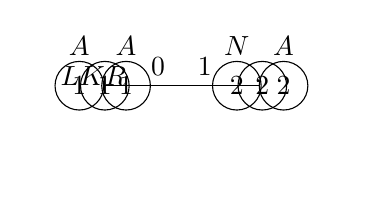
\begin{tikzpicture} 
                    \graphbox{\( L \)}{-40mm}{-3mm}{34mm}{15mm}{-8mm}{-9mm}{
                        \node[draw, circle] (x) at (0,0) {1};  
                        \node[draw, circle] (y) at (2,0) {2};
                        \draw[-] (x) -- node[midway,above] {0} (y) ;
                        \node  () at (0,0.5) {$A$};  
                        \node () at (2,0.5) {$N$};
                    } 
                    \graphbox{\( K \)}{0mm}{-3mm}{34mm}{15mm}{-8mm}{-9mm}{
                        \node[draw, circle] (x) at (0,0) {1};  
                        \node[draw, circle] (y) at (2,0) {2};
                    } 
                    \graphbox{\( R \)}{40mm}{-3mm}{34mm}{15mm}{-8mm}{-9mm}{
                        \node[draw, circle] (x) at (0,0) {1};  
                        \node[draw, circle] (y) at (2,0) {2};
                        \draw[-] (x) -- node[midway,above] {1} (y) ;
                        \node  () at (0,0.5) {$A$};  
                        \node () at (2,0.5) {$A$};
                    }  
                    \node () at (37mm,-10mm) {\( \rightarrowtail \)}; % K -> L
                    \node () at (-3mm,-10mm) {\( \leftarrowtail  \)}; % K -> L
                \end{tikzpicture}
    \caption{}
    \label{fig:intro:graph_transformation_rule_0_dpo}
    \end{figure}
    
Since graph transformation rules in a system are applied repeatedly and nondeterministically, they can lead to infinite sequences of graph transformations. For example, consider the rewriting rule in~\autoref{fig:intro:graph_transformation_rule_nonterminating} replaces an occurrence of the graph \tikz[baseline=-0.5ex]{ 
        \node (x) at (0,0) {$\bullet$};  
        \node (y) at (1,0) {$\bullet$};
        \node (z) at (2,0) {$\bullet$};
        \draw[->] (x) -- node[midway,below] {a} (y) ;
        \draw[->] (y) -- node[midway,below] {b} (z) ;
} by that of the graph \tikz[baseline=-0.5ex]{ 
        \node (x) at (0,0) {$\bullet$};  
        \node (y) at (1,0) {$\bullet$};
        \node (z) at (2,0) {$\bullet$};
        \draw[->] (x) -- node[midway,below] {b} (y) ;
        \draw[->] (y) -- node[midway,below] {a} (z) ;
} while keeping the extreme nodes unchanged.
    \begin{figure}[!htbp]
        \centering
            \resizebox{0.85\textwidth}{!}{
                \begin{tikzpicture}[baseline=-3ex]
                    \graphbox{\( L \)}{0mm}{-3mm}{34mm}{15mm}{2mm}{2mm}{
                        \coordinate (o) at (0mm,-11mm); 
                        \node[draw,circle] (l1) at ($(o)+(-10mm,0mm)$) {1};
                        \node[draw,circle] (l2) at ($(l1)+(2,0)$) {2};
                        \node[draw,circle] (l3) at ($(l1) + (1,0)$) {3};
                        \draw[->] (l1) -- (l3) node[midway,above] {a};
                        \draw[->] (l3) -- (l2) node[midway,above] {b};
                    } 
            
                    \graphbox{\( K \)}{40mm}{-3mm}{34mm}{15mm}{2mm}{2mm}{
                        \coordinate (o) at (0mm,-11mm); 
                        \node[draw,circle] (l1) at ($(o)+(-10mm,0mm)$) {1};
                        \node[draw,circle] (l2) at ($(l1)+(2,0)$) {2};
                    }  
            
                    \graphbox{\( R \)}{80mm}{-3mm}{35mm}{15mm}{2mm}{2mm}{
                        \coordinate (o) at (-5mm,-11mm); 
                        \node[draw,circle] (l1) at ($(o)+(-10mm,0mm)$) {1};
                        % \node[draw,circle] (l2) at ($(l1)+(3,0)$) {2};
                        \node[draw,circle] (l3) at ($(l1) + (1,0)$) {4};
                        \node[draw,circle] (l4) at ($(l1) + (2,0)$) {2};
                        \draw[->] (l1) -- (l3) node[midway,above] {b};
                        \draw[->] (l3) -- (l4) node[midway,above] {a};
                        % \draw[->] (l4) -- (l2) node[midway,above] {a};
                    }    
                    \node () at (37mm,-10mm) {\( \leftarrowtail \)}; % K -> L
                    \node () at (77mm,-10mm) {\( \rightarrowtail \)}; % K -> R
                \end{tikzpicture}
                }
        \caption{}
        \label{fig:intro:graph_transformation_rule_nonterminating}
    \end{figure}
    A looping rewriting sequence using the rule in~\autoref{fig:intro:graph_transformation_rule_nonterminating}, where the graph is in a box with it name on the top left corner, numbers inside nodes are used to identify them, can be visualized as in~\autoref{fig:intro:sequence_of_transformation_infinite} with matches in red.

        \begin{figure}[!htbp]
            \centering
          \resizebox{0.85\textwidth}{!}{
            \tikz
            [baseline=-0.5ex]
            { 
                \node (x) at (0,0) {$\bullet$};  
                \node (y) at (1,0) {$\bullet$};
                \node (z) at (0.5,0.86) {$\bullet$};
                \draw[->,red] (x) -- node[midway,below] {a} (y) ;
                \draw[->,red] (y) -- node[midway,right] {b} (z) ;
                \draw[->] (z) -- node[midway,left] {b} (x) ;
            } 
            $\Rightarrow$ 
            \tikz[baseline=-0.5ex]{ 
                \node (x) at (0,0) {$\bullet$};  
                \node (y) at (1,0) {$\bullet$};
                \node (z) at (0.5,0.86) {$\bullet$};
                \draw[->] (x) -- node[midway,below] {b} (y) ;
                \draw[->,red] (y) -- node[midway,right] {a} (z) ;
                \draw[->,red] (z) -- node[midway,left] {b} (x) ;
            }
            $\Rightarrow$ 
            \tikz[baseline=-0.5ex]{ 
                \node (x) at (0,0) {$\bullet$};  
                \node (y) at (1,0) {$\bullet$};
                \node (z) at (0.5,0.86) {$\bullet$};
                \draw[->,red] (x) -- node[midway,below] {b} (y) ;
                \draw[->] (y) -- node[midway,right] {b} (z) ;
                \draw[->,red] (z) -- node[midway,left] {a} (x) ;
            }
            $\Rightarrow$ 
            \tikz[baseline=-0.5ex]{ 
                \node (x) at (0,0) {$\bullet$};   
                \node (y) at (1,0) {$\bullet$};
                \node (z) at (0.5,0.86) {$\bullet$};
                \draw[->,red] (x) -- node[midway,below] {a} (y) ;
                \draw[->,red] (y) -- node[midway,right] {b} (z) ;
                \draw[->] (z) -- node[midway,left] {b} (x) ;
            }
          }
          \caption{}
          \label{fig:intro:sequence_of_transformation_infinite}
        \end{figure}
    It is crucial to ensure that a rewriting system cannot transform a graph indefinitely, in order to discuss the output of that rewriting system, because otherwise the output is undefined. This leads to the problem of termination.

\paragraph{Termination} is a property of DPO graph rewriting systems. It ensures that no graph can be transformed indefinitely under a given set of rewriting rules. For example, the rule in~\autoref{fig:intro:graph_transformation_rule} terminates because each application reduces the number of nodes in a graph by one, and the rule in~\autoref{fig:intro:graph_transformation_rule_nonterminating} does not terminate.
Many termination techniques exist for term rewriting systems~\cite{nipkow1998term, dershowitz1982orderings, middeldorp1997simple, arts2000termination}.  
Most exploit the tree structure of terms—a feature absent in general graphs—making direct adaptation impossible. 
% ,dick1990automating,giesl1995generating,zantema1994termination,bellegarde1990termination,zantema1995termination
% These techniques prove the termination of a rewriting system by embedding the binary relations defined by a term rewriting system onto a well-founded order. This is done either explicitly or implicitly. 
% In the cases, for example , one defines explicitly a well-founded order on terms, and then proves that terms can be interpreted as elements of the well-founded order, and that the application of a rule transforms a term into another term that is smaller than the original term in the well-founded order~\cite{.
% In the latter case, one defines a well-founded order on terms, and then proves that the application of a rule transforms a term into another term that is smaller than the original term in the well-founded order. In this case,
% the technique is classified as \enquote{techniques by interpretation} in the literature, and in the latter case, they are classified as \enquote{syntactic techniques}, \enquote{techniques by dependencies pairs}, \enquote{semantic labelling}, \enquote{hierarchical termination}, etc. \todo{references and explanation}
Therefore, new techniques are needed for proving termination of DPO graph rewriting systems. However, developing termination techniques for rewriting systems is difficult, because a system may have many rules, and, therefore, many constraints on the behavior of the rules must be satisfied. A more interesting approach is to prove that the system in question can be separated into two disjoint subsets of rules, one of which can be applied only finitely many times in any sequence using rules from the union of the two sets, thus the termination of the system can be reduced to the termination of the other set of rules. This leads to the concept of relative termination.

\paragraph{Relative termination} is a concept introduced by Klop in~\cite{klop1987term}. It generalizes the termination property.
 Given two rule sets \( \mathcal{A} \) and \( \mathcal{B} \), relative termination of \( \mathcal{A} \) with respect to \( \mathcal{B} \) ensures that, for any finite graph $G$,
rules in $\mathcal{A}$ can only be applied finitely many times in any sequence of rule applications from $\mathcal{A} \cup \mathcal{B}$.
% Intuitively, this property corresponds to the phenomenon that while some distributed systems do not halt for every input, some of their operations can only be applied finitely many times in any execution. 
% Therefore, these operations do not need to be considered when reasoning about the termination of the system. The problem to be analyzed can thus be simplified by safely ignoring these operations.
  
Consider the graph transformation system with two rules illustrated in~\autoref{fig:intro:edge_deletion_and_node_addition_rule}: rule $\alpha$ deletes an arbitrary edge labeled by \enquote{a} and rule $\beta$ introduces a fresh node.
  \begin{figure}[!htbp]
        \centering
%   \begin{subfigure}{0.3\textwidth}
%         % \centering
        $\alpha$ = {
            \begin{tikzpicture}
                        \graphbox{\( L \)}{0mm}{-3mm}{34mm}{15mm}{2mm}{2mm}{
                            \coordinate (o) at (0mm,-11mm); 
                            \node[draw,circle] (l1) at ($(o)+(-10mm,0mm)$) {1};
                            \node[draw,circle] (l2) at ($(l1)+(2,0)$) {2};
                            \draw[->] (l1) -- (l2) node[midway,above] {a};
                        } 
                        \graphbox{\( R \)}{40mm}{-3mm}{34mm}{15mm}{2mm}{2mm}{
                            \coordinate (o) at (0mm,-11mm); 
                            \node[draw,circle] (l1) at ($(o)+(-10mm,0mm)$) {1};
                            \node[draw,circle] (l2) at ($(l1)+(2,0)$) {2};
                        }  
                        \node () at (37mm,-10mm) {\( \rightarrowtail \)}; % K -> L
                    \end{tikzpicture}
                    }
    %     \caption{A graph transformation rule for edge deletion}
    % \label{fig:intro:edge_deletion_rule}
    % \end{subfigure}
    
    % \begin{subfigure}{0.3\textwidth}
    %     % \centering

        $\beta$ ={
            \begin{tikzpicture}
                        \graphbox{\( L \)}{0mm}{-3mm}{34mm}{15mm}{2mm}{2mm}{

                        } 
                        \graphbox{\( R \)}{40mm}{-3mm}{34mm}{15mm}{2mm}{2mm}{
                            \coordinate (o) at (0mm,-11mm); 
                            \node[draw,circle] (l1) at ($(o)+(5mm,0mm)$) {};
                        }  
                        \node () at (37mm,-10mm) {\( \rightarrowtail \)}; % K -> L
                    \end{tikzpicture}
                    }
    %     \caption{A graph transformation rule for node addition}
    %     \label{fig:intro:node_addition_rule}
    % \end{subfigure}
    \caption{A rewriting system}
    \label{fig:intro:edge_deletion_and_node_addition_rule}
  \end{figure}
  This system does not terminate, as the node-adding rule $\beta$ can be applied indefinitely. However, the relative termination of the edge-deletion rule $\alpha$ with respect to the node-adding rule $\beta$ can be established, because the initial graph is finite, and neither rule increases the number of edges in the graph.
   Consequently, termination of the full system reduces to the termination of the subsystem consisting of the node-adding rule $\beta$.

  This approach has several advantages.
  Firstly, it allows us to reduce the size of the system to be analyzed. Secondly, different techniques can cooperate in a straightforward way, leveraging the strengths of each technique, because at each iteration of the analysis, we can try different techniques.
   Thirdly, combined with Plump's modular termination technique~\cite{plump2018modular}, which proves termination of a system by establishing termination for two rule sets that partition the system's rules, the termination analysis of DPO graph rewriting systems can be much easier.

\paragraph{Termination of DPO graph rewriting systems on edge-labeled directed multigraphs} is the focus of this thesis, even though, using the language of category theory, it is possible to develop termination techniques for DPO rewriting systems on different graph notions that satisfy certain properties. There are several reasons for this choice.

First of all, edge-labeled directed multigraphs are simple and intuitive: they are just directed graphs with multiple edges between two nodes allowed, and each edge is labeled by a symbol from a finite alphabet. This notion of graph is widely used in the literature, such as in the work introducing the DPO graph rewriting~\cite{ehrig1973graph}, in previous work on the method that we extend in~\autoref{chap:nwf}~\cite{bruggink2014termination,bruggink2015proving,zantema2014termination}, and in illustrative examples of works~\cite{overbeek2024termination_lmcs,endrullis2024generalized_icgt} which are closely related to our work in Chapter~\autoref{chap:subgraph_counting} and Chapter~\autoref{chap:antipattern}.

 Secondly, by focusing on this notion of graph, we want to avoid overly abstract reasoning and make the techniques more accessible to users than those based on more abstract notions of graph, such as adhesive categories~\cite{lack2004adhesive}.
 As a consequence, the correctness of our technique in Chapter~\ref{chap:subgraph_counting} and Chapter~\ref{chap:antipattern} can be checked easily by users with basic knowledge in graph theory and very basic knowledge in category theory, and thus users can adopt it with real confidence.
 We believe that automated tools should be easy
to understand by users without
spending too much time. Otherwise, they can only trust the author of the tool
or not use the tool at all\textemdash either of which is in conflict with the very essence of verification.  

% Finally, by sticking to a specific notion of graph, we can exploit the properties that are specific to that notion of graph. This leads to more powerful termination techniques. Since termination of DPO graph rewriting systems is undecidable in general~\cite{plump1998terminationundecidable}. It is important to push as far as possible the boundaries of what can be achieved with termination techniques for DPO graph rewriting systems.

Finally, specializing to edge-labeled directed multigraphs enables us to leverage graph-specific properties to develop stronger termination criteria. Because termination is undecidable for general DPO graph rewriting systems~\cite{plump1998terminationundecidable}, this specialization is essential for extending the boundaries of practically verifiable termination. 

\paragraph{Existing techniques}
Few techniques for proving (relative) termination of DPO graph rewriting systems exist. Below, we list some of the existing techniques.

\begin{itemize}
    \item Overbeek and Endrullis developed a termination technique for PBPO+ graph rewriting systems~\cite{overbeek2024termination_lmcs}. This technique counts the number of occurrences of certain subgraphs before and after a rewriting step. This technique can be applied to PBPO+ graph rewriting systems on many categories including edge-labeled directed multigraphs. It can also be applied to left-injective DPO graph rewriting systems.
    \item The type graph method, which weighs an object by summing the weights of morphisms from the object to a type graph, was initially introduced by Zantema, K{\"o}nig and Bruggink~\cite{zantema2014termination} for cycle-rewriting systems. 
    This method has since been generalized to edge-labeled multigraphs by Bruggink et al.~\cite{bruggink2014termination} for DPO rewriting with monic matches and injective rules, later extended to DPO rewriting in general by Bruggink et al.~\cite{bruggink2015proving}, and further adapted to more categories and different DPO variants by Endrullis et al.~\cite{endrullis2024generalized_arxiv_v2}. 
    \item Plump~\cite{plump1995ontermination} introduced a necessary and sufficient termination condition for left-injective DPO hypergraph rewriting via forward closure, though verifying this condition is undecidable. 
    \item Plump~\cite{plump2018modular} later proposed a modular critical pair-based strategy for left-injective DPO hypergraph rewriting with monic matches. It allows to deduce termination of the union of two systems from the termination of their sub-systems.
    % \item Levendovszky et al.~\cite{levendovszky2007termination} propose a termination criterion for DPO rewriting (monic matches, injective rules, negative application condition), though automated verification is hard as explained in~\cite[\textsection 6]{levendovszky2007termination}. 
    % \item Bottoni et al.~\cite{bottoni2005termination} propose a termination criterion for DPO/SPO rewriting on high-level replacement units. Their method imposes a strongly constrained measuring function and the only concretes measuring function proposed are node-counting and edge-counting.
    % \item Bottoni et al.~\cite{bottoni2010atermination} present a criterion for termination of DPO rewriting with monic matches, injective rules and negative application conditions, based on the construction of a labeled transition system. 
\end{itemize}

\paragraph{Contribution 1: Termination of Graph Rewriting Using Weighted Type Graphs over Non-well-founded Semirings}
While the weighted type graph method is a powerful technique for proving termination of double-pushout (DPO) graph rewriting systems, existing approaches require weighted type graphs to have weights over well-founded semirings. This approach has practical limitations when applied to edge-labeled directed multigraph rewriting. Chapter~\ref{chap:nwf} investigates the use of non-well-founded semirings to overcome these limitations. 
% Chapter~\ref{chap:nwf} is based on the following paper:
% \begin{itemize}
%     \item Qi Qiu. Termination of Graph Rewriting using Weighted Type Graphs over Non-well-founded Semirings. 16th International Workshop on Graph Computation Models, Jun 2025, Koblenz, Germany. 2025. ⟨hal-04954960v3⟩
% \end{itemize}
 
\paragraph{Contribution 2: Termination of Injective DPO Graph Rewriting Systems Using Subgraph Counting} 
To resolve some cases that prior interpretation-based methods cannot handle, Chapter~\ref{chap:subgraph_counting} presents a new machine-checkable sufficient condition for relative termination of DPO graph rewriting systems with injective rules on edge-labeled multigraphs. 
It is based on the idea that if the number of a specific subgraph in the graph strictly decreases every time a transformation is performed, then the transformation cannot last indefinitely.
The method defines a graph's weight as the sum of weights of occurrences of a set of graphs within it. Given two rule sets A and B, by ensuring 
(1) every rewriting step using rules in A strictly decreases the host graph's weight and 
(2) every rewriting step using rules in B never increases it, we guarantee that rules in A can be applied only finitely many times in any rewriting sequence using rules from the union of A and B. 
% Chapter~\ref{chap:subgraph_counting} is based on the following paper:
% \begin{itemize}
%     \item Qiu, Q. (2025). Termination of Injective DPO Graph Rewriting Systems Using Subgraph Counting. In: Endrullis, J., Tichy, M. (eds) Graph Transformation. ICGT 2025. Lecture Notes in Computer Science, vol 15720. Springer, Cham. \url{https://doi.org/10.1007/978-3-031-94706-3_1}
% \end{itemize}

\paragraph{Contribution 3: Termination of Injective DPO Graph Rewriting Systems Using Subgraph Counting with Antipattern}
The termination property of a graph rewriting system can sometimes be established by analyzing a decrease in the number of occurrences of specific subgraphs that are not embedded within forbidden contexts. For example, consider the DPO graph rewriting rule in~\autoref{fig:intro:graph_transformation_rule_anti_pattern}.
 \begin{figure}[!htbp]
    \centering
\begin{tikzpicture}
      \graphbox{$L$}{0mm}{0mm}{34mm}{20mm}{2mm}{-5mm}{
          \coordinate (o) at (0mm,-3mm); 
          \node[draw,circle] (l1) at ($(o)+(-10mm,0mm)$) {1};
          \node[draw,circle] (l2) at ($(l1)+(2,0)$) {2};
          \node[draw,circle] (l3) at ($(l1) + (1,0)$) {3};
          \draw[->] (l1) -- (l3) node[midway,above] {a};
          \draw[->] (l3) -- (l2) node[midway,above] {a};
      }     
      \graphbox{$K$}{40mm}{0mm}{24mm}{20mm}{2mm}{-5mm}{
          \coordinate (o) at (5mm,-3mm); 
          \node[draw,circle] (l1) at ($(o)+(-10mm,0mm)$) {1};
          \node[draw,circle] (l2) at ($(l1)+(1,0)$) {2};
      }    
      \graphbox{$R$}{70mm}{0mm}{45mm}{20mm}{2mm}{-5mm}{
        \coordinate (o) at (0mm,-3mm); 
        \node[draw,circle] (l1) at ($(o)+(-10mm,0mm)$) {1};
        \node[draw,circle] (l2) at ($(l1)+(2,0)$) {2};
        \node[draw,circle] (l3) at ($(l1) + (1,0)$) {3};
        \draw[->] (l1) -- (l3) node[midway,above] {a};
        \draw[->] (l3) -- (l2) node[midway,above] {a};
        \draw[->] (l3) edge [loop below] node {$c$} (l3);
      }    

      \node () at (37mm,-10mm) {$\leftarrowtail$};
      \node () at (67mm,-10mm) {$\rightarrowtail$};
  \end{tikzpicture}
  \caption{}
  \label{fig:intro:graph_transformation_rule_anti_pattern}
 \end{figure}

 
Each application of this rule reduces the number of occurrences of the left-hand side graph $L$ that are not included in any occurrence of the right-hand side graph $ R $. While this variant suggests termination, existing subgraph counting methods (e.g., those in Chapter~\ref{chap:subgraph_counting} and~\cite{overbeek2024termination_lmcs}) cannot exploit such relationships to infer termination. In this chapter, we extend the subgraph counting framework introduced in Chapter~\ref{chap:subgraph_counting} to address systems of this kind.

The extension successfully proves termination for systems like the ones presented in~\autoref{antipattern:ex:grs_aca} and~\autoref{antipattern:ex:endrullis:d3:termination} which prior approaches~\cite{zantema2014termination,bruggink2014termination,bruggink2015proving,endrullis2024generalized_arxiv_v2,overbeek2024termination_lmcs} and the subgraph counting method presented in Chapter~\ref{chap:subgraph_counting} fail to handle. 

\paragraph{Contribution 4: LyonParallel}
We developed a termination tool for DPO edge-labeled multigraph rewriting that integrates the existing type graph method, our extension, and our subgraph counting technique and its extension.